\section{Mechanics}
% In this section briefly describe the software and hardware of the robot
\setlength\intextsep{0pt}
In the past two years there were multiple changes applied to the chip kicker in order to reach the most efficient design. A great number of simulation tests were done on every chip design and after a successful test, the parts were manufactured for real world testing procedures.

\subsection{Chip kickers new design}
Chip kicker is a part which should have a high resistance against impacts, It has to be efficient in transmitting the force applied to it from the chip kicker plunger to the ball. The first improvement in the chip kicker is that $\theta$ (angle between a line which passes through the chip kickers axis of rotation and impact point and the direction of the force vector)has been increased to 90 degrees. With this improvement the force applied to the chip kicker will be completely in the direction of the angular acceleration of the chip kicker. According to the torque relation, It is shown that when the angle between the force and the distance vector turn into 90 degrees, The ball would receive the most impact from that force.\\
\indent The other improvement is to increase the moment of inertia around the chip kickers axis of rotation. This way, more angular acceleration can be achieved by the chip kicker.\\
\indent In this section we will derive a function for angular acceleration of the chip kicker. As known, the relation between the moment of inertia around the chip kickers axis of rotation and sum of torque applied to the chip kicker can be written as:
\begin{equation}
\sum T=I\alpha
\end{equation}
\begin{equation}
T=Fb
\end{equation}
Where b is the vertical distance between the center of the chip kickers pin and the point which force is applied.\\
It is not necessary to calculate the impact force accurately thus, it is assumed that the force applied, is constant to reduce the parameters involved in the new chip kickers design. the impact force is approximated by the equation below:
\begin{equation}
F=\dfrac{m\limits_{plunger} {V}^2\limits_{f-plunger}}{2d}
\end{equation}
Where $m\limits_{plunger}$ is the mass of the plunger and ${V}\limits_{f-plunger}$ is the velocity of plunger exactly before the impact and $d$ is the distance in which the plunger and the chip kicker are in contact during the impact.\\
\indent Below is an expression for the angular acceleration, resulted from the previous equations:
\begin{equation}
\alpha = \dfrac{b m\limits_{plunger} {V}^2\limits_{f-plunger}}{2Id}
\end{equation}
By assuming F as constant, The angular acceleration will be a function of:
\begin{equation}
\alpha=f(\dfrac{b}{I})
\end{equation}
As a result, if the moment of inertia around the axis of rotation reduces by decreasing the mass of the chip kicker or reducing the distance between its center of mass and the axis of rotation, $\alpha$ will increase.
As shown in Fig.\ref{fig:CHIP_SIDE_VIEW}, $\dfrac{b}{I}$ is calculated for both old and new designs:\\
\begin{figure}
	\centering
	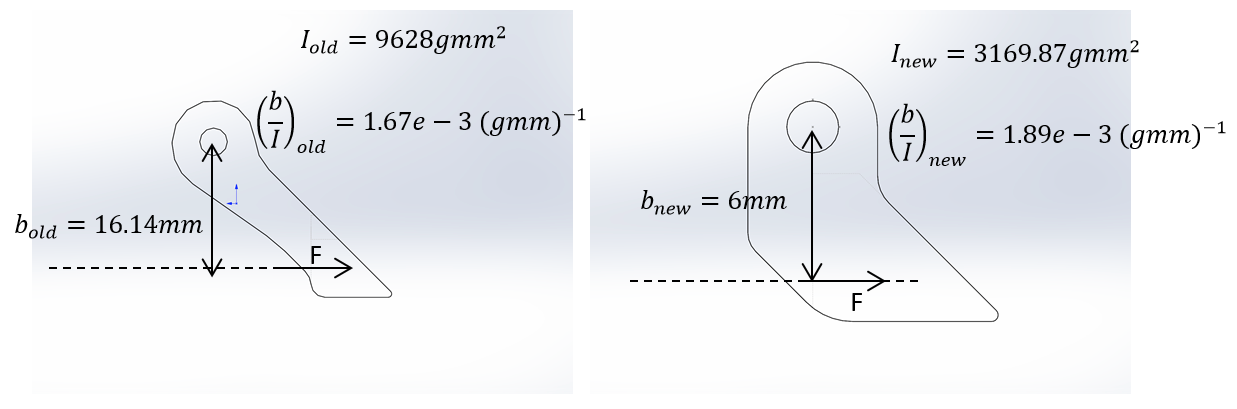
\includegraphics[width=1.0\textwidth]{images/SIDE_VIEW_CHIP.png}
	\caption{$\dfrac{b}{I}$ for old (left) and new (right) design}
	\label{fig:CHIP_SIDE_VIEW}
\end{figure}\\
The results show that $\dfrac{b}{I}$ for the new design is larger than the old one; Therefore, the angular acceleration for the new design should be more than the angular acceleration in the old design. As discussed above, the new design of the chip kicker is much more simple to manufacture ,more reliable and lighter than the old design. %Including these improvements, it also has higher angular acceleration which means reducing its weight won’t affect its functionality.\\
\\
\indent In order to test these results, the impact for both old and new designs were simulated in solid works (as shown in Fig.\ref{fig:SIM2CHIP}).\\
\begin{figure}
	\centering
	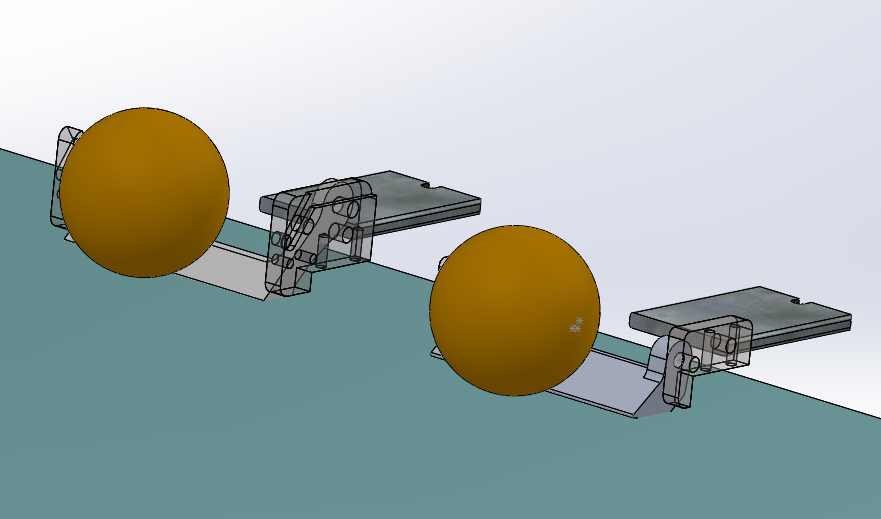
\includegraphics[width=0.8\textwidth]{images/SIM_CHIPx2.png}
	\caption{A view of the old (top left)and new (bottom right)chip kickers in a simulation enviroment}
	\label{fig:SIM2CHIP}
\end{figure}\\
\\
The new chip kicker was tested in a standard SSL field. The results can be seen and compared in Fig. \ref{fig:NEWOLDPLOTBALL}.\\
\begin{figure}
	\centering
	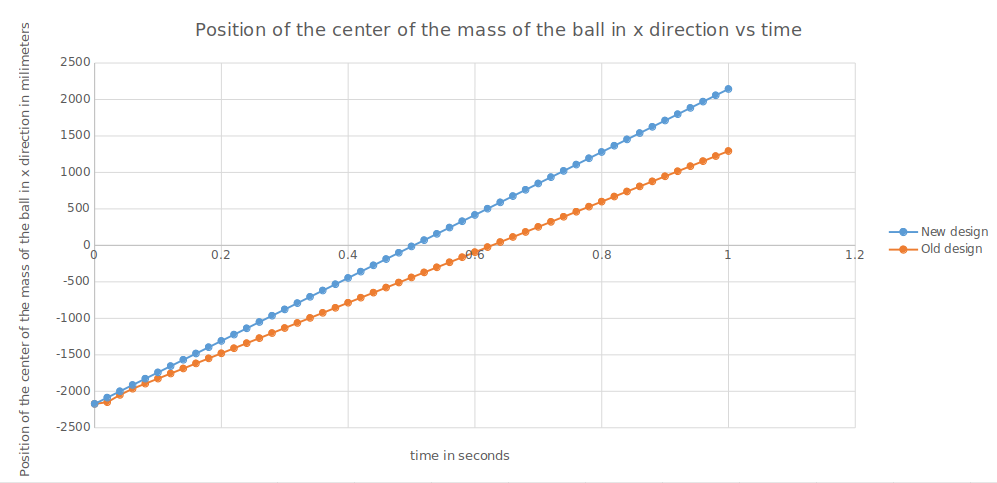
\includegraphics[width=0.8\textwidth]{images/CHIP_POS_PLOT.png}
	\caption{Position time graph for a ball being kicked by the new chip kicker (Blue)and old chip kick(Orange)}
	\label{fig:NEWOLDPLOTBALL}
\end{figure}
%\begin{figure}
%	\centering
%	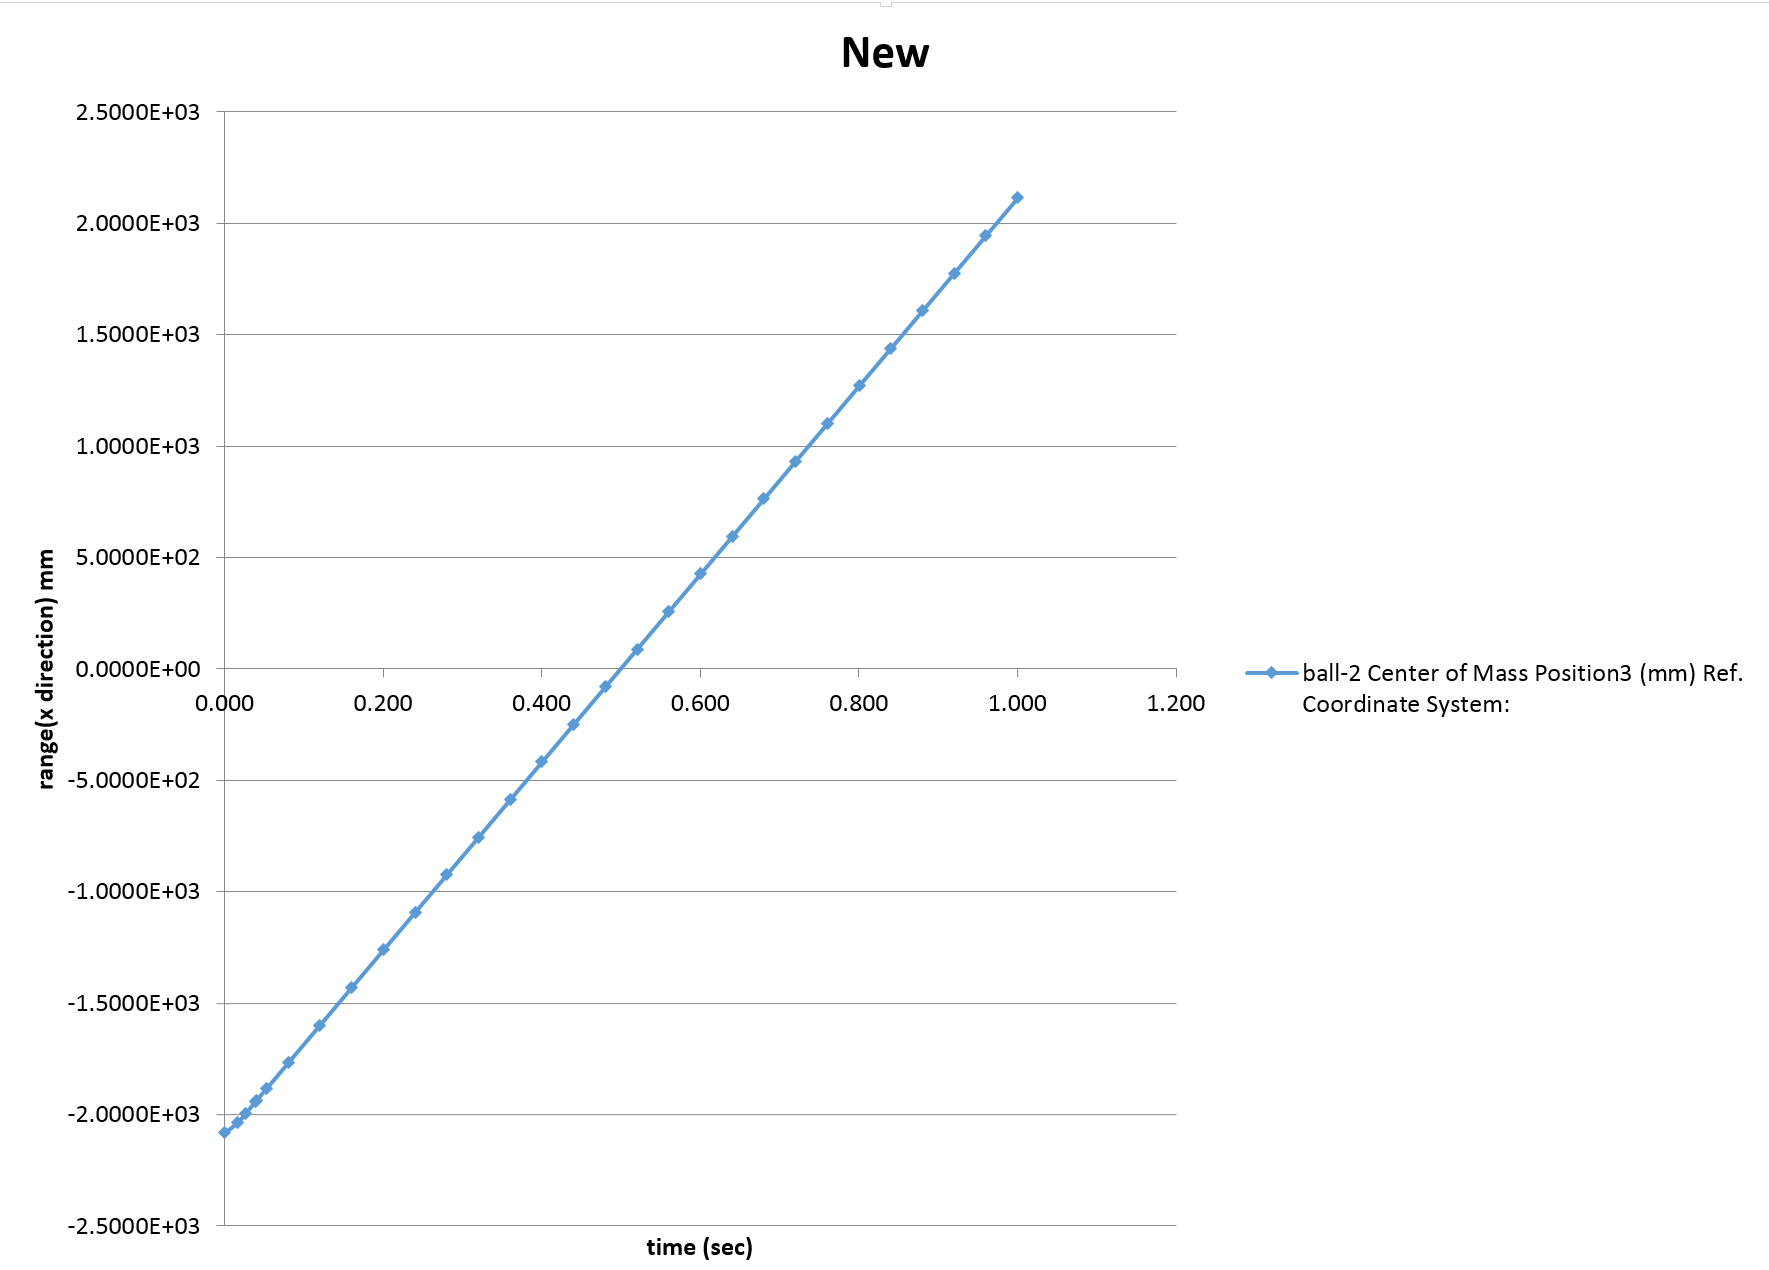
\includegraphics[width=0.8\textwidth]{images/NewBallPlot.png}
%	\caption{Position time graph for a ball being kicked by the new chip kicker}
%	\label{fig:NEWPLOTBALL}
%\end{figure}\\
%\begin{figure}
%	\centering
%	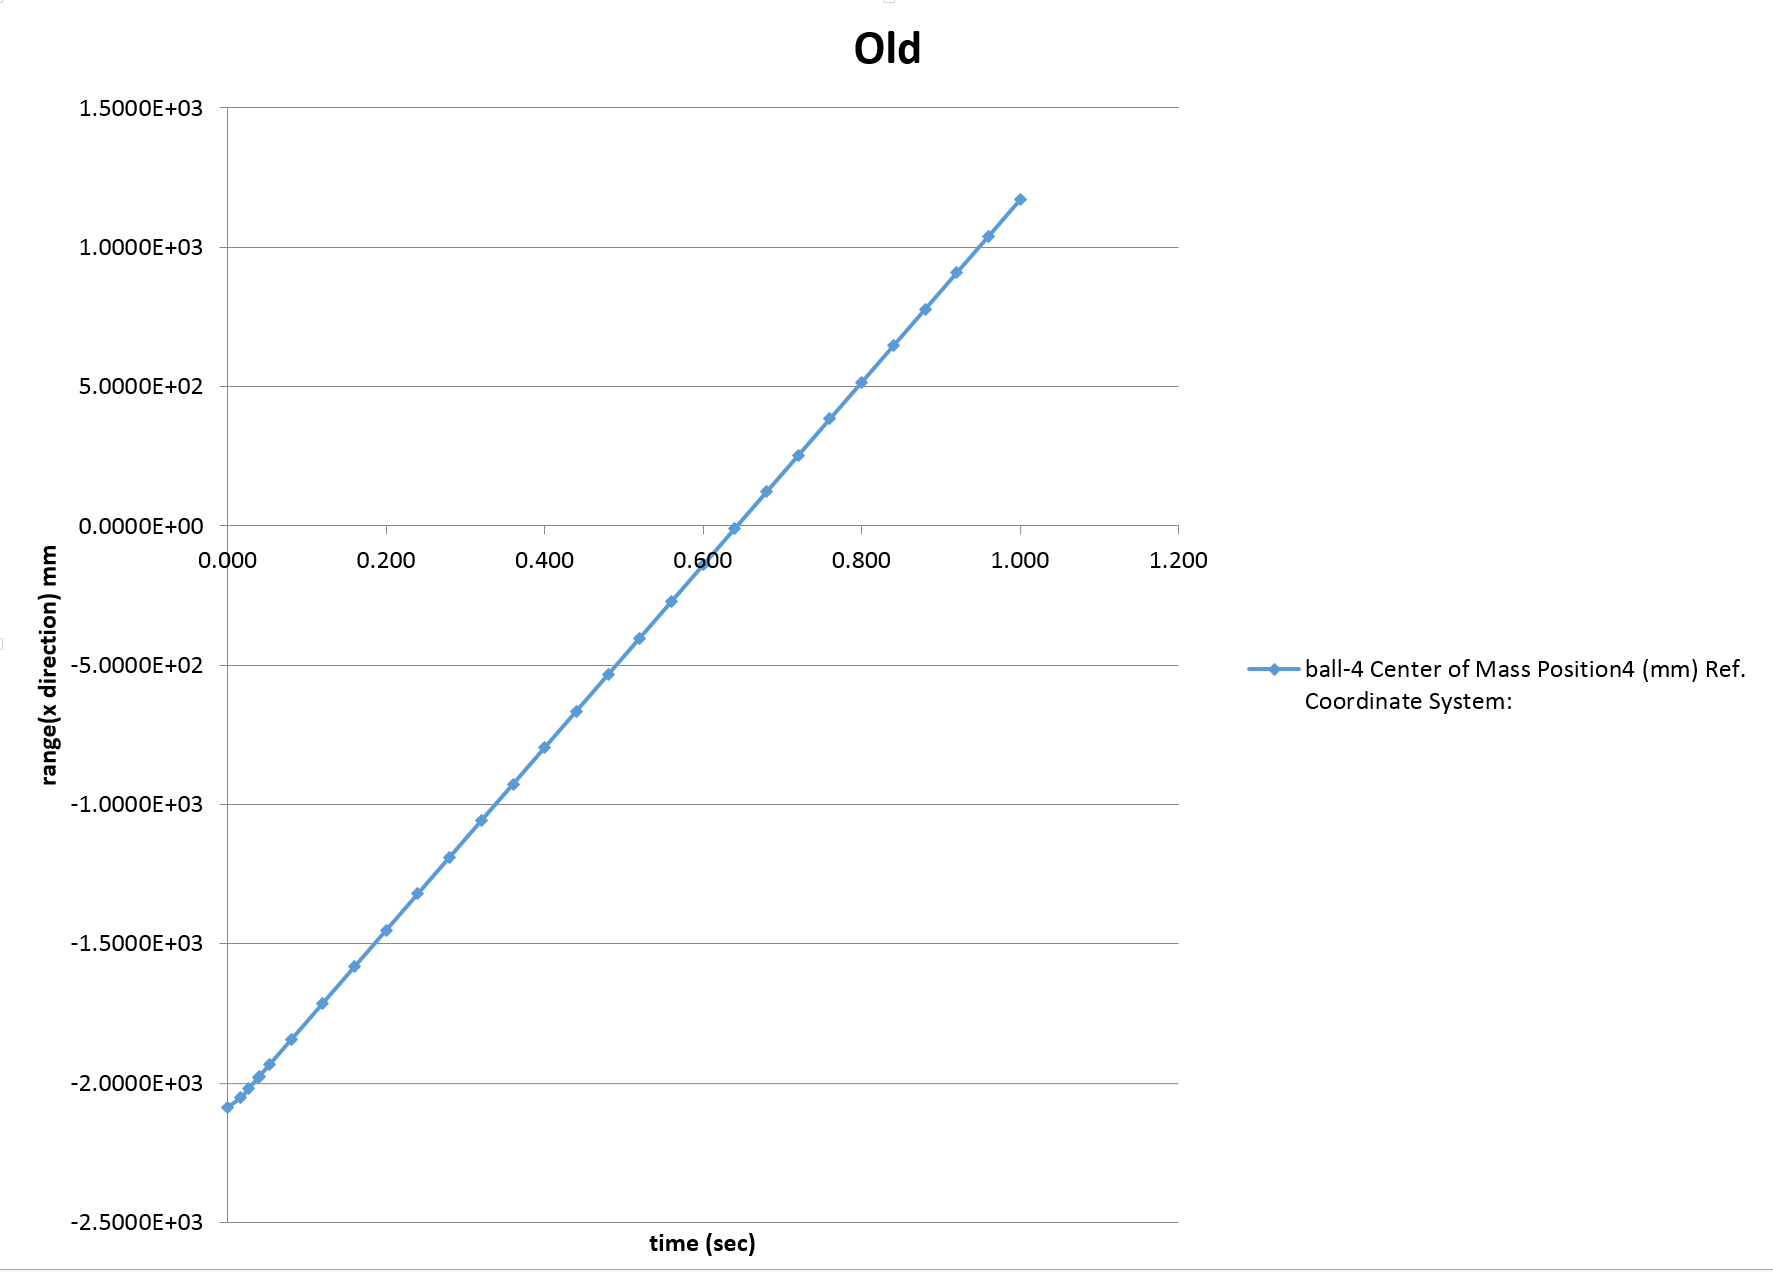
\includegraphics[width=0.8\textwidth]{images/OldBallPlot.png}
%	\caption{Position time graph for a ball being kicked by the old chip kicker}
%	\label{fig:OLDPLOTBALL}
%\end{figure}\\
\\
In conclusion, the new chip kicker can kick the ball further than the old one. The most important point here is that the new chip kickers design made its process of manufacturing much easier and faster. %Also new design of kicking device is in a way that it can be easily disassembled from the robot which makes its repair process much faster. Faster robot repairing means having more robots operate when the match is taking place.



